% =============================================================================
% Chapter 4: Semantic Annotation Approaches
% =============================================================================
\chapter{Semantic Annotation Approaches}
\label{chap:semantic_annotation_approaches}
Energy datasets pose distinctive challenges for semantic annotation, including terminological inconsistency across data providers, deeply hierarchical concept taxonomies, and limited standardization of naming conventions. Addressing these issues requires a principled framework that couples ontology-guided search with robust semantic inference.
Pan et al. (2025)~\cite{pan2025semantic} propose a pipeline that combines ontology-driven traversal with large language model (LLM) reasoning and ensemble aggregation; the remainder of this chapter formalizes and analyzes that pipeline. Section~\ref{sec:problem_formulation} defines Column Type Annotation (CTA) for energy tables and introduces notation. Section~\ref{sec:bfs} describes an ontology-driven breadth-first search strategy for candidate generation. Section~\ref{sec:prompt_engineering} specifies the prompting procedure that constrains LLM outputs to ontology-consistent labels. Section~\ref{sec:edm} presents an ensemble decision-making module that aggregates multiple model judgments to improve robustness.

\section{Problem Formulation}
\label{sec:problem_formulation}

Semantic annotation augments raw data with metadata that links records to concepts defined in an ontology or knowledge base~\cite{jimenez2020semtab}. For tables, the literature commonly distinguishes three subtasks: Cell Entity Annotation (CEA), which disambiguates individual cell values to knowledge-base entities; Column Property Annotation (CPA), which identifies semantic relations between columns; and Column Type Annotation (CTA), which assigns one or more ontological classes to a column based on its values.

This thesis targets CTA for energy datasets. Unlike conventional database-to-ontology alignment that maps columns to binary predicates, CTA associates each column directly with one or more ontological classes. This formulation matches the granularity of many energy tables, where columns often encode standalone domain concepts (e.g., \textit{Fuel Type}, \textit{Energy Source}, \textit{Region}) that align more naturally with class definitions than with relational properties.

Formally, let $\mathcal{T}=\{t_1, t_2, \cdots, t_n\}$ denote a set of tables, where each table $t_i$ contains a set of columns $\mathcal{C}_i=\{c_{i,1}, c_{i,2}, \cdots, c_{i,j}\}$. Semantic annotation maps each column $c_{i,j}$ to a class or set of classes in a predefined ontology $\mathcal{O}=\{o_1, o_2, \cdots, o_m\}$, thereby standardizing semantic representation across heterogeneous datasets. Let $\mathcal{M}$ denote the mapping function, where $\mathcal{C}=\bigcup_{i=1}^{n}\mathcal{C}_i$ is the universe of columns and $\mathcal{P}(\mathcal{O})$ is the power set of classes:

\begin{equation}
\mathcal{M}: \mathcal{C} \rightarrow \mathcal{P}(\mathcal{O}), \quad \text{where } \mathcal{M}(c_{i,j}) =
\begin{cases}
\{o_s\}, & \text{a single class,} \\
\{o_{s_1}, o_{s_2}, \cdots\} \subset \mathcal{O}, & \text{multiple classes,} \\
\emptyset, & \text{no assigned class.}
\end{cases}
\end{equation}

Heterogeneous column naming conventions and domain-specific terminology complicate this mapping: semantically equivalent concepts may appear under divergent headers. Consequently, the objective is to construct $\mathcal{M}$ such that each column $c$ is assigned the ontological classes $o$ for which the similarity score $\mathcal{S}(c,o)$ exceeds a threshold $\tau$, where $\mathcal{S}: \mathcal{C} \times \mathcal{O} \rightarrow [0, 1]$ quantifies the semantic affinity between $c$ and $o$.

\begin{equation}
\mathcal{M}(c)=\{o \in \mathcal{O} \mid \mathcal{S}(c, o) \ge \tau\}
\end{equation}

Pan et al. (2025) address this matching problem through a three-stage pipeline that couples ontology-driven traversal with LLM-based reasoning (Figure~\ref{fig:methods_ontology_bfs_pipeline})~\cite{pan2025semantic}. An Ontology-Driven Breadth-First Search (BFS) algorithm navigates the ontology hierarchy level by level, generating candidate classes at each depth. For every set of candidates, a structured prompt supplies table context, including column headers and sampled cell values, to elicit semantic judgments from multiple LLM instances. An Ensemble Decision-Making (EDM) module then aggregates these judgments via majority voting, retaining only those classes that surpass a consensus threshold. The surviving candidates are enqueued for further refinement at deeper hierarchy levels, and the process iterates until terminal classes are reached. The following sections detail each component in turn.

\begin{figure}[ht]
    \centering
    \includegraphics[width=\textwidth]{graphics/canvas/methods.pdf}
    \caption{Workflow of the semantic annotation pipeline. The Ontology-Driven BFS module traverses the ontology DAG and dispatches candidate classes together with table context to an LLM-based EDM module, which returns consensus-selected classes for subsequent traversal.}
    \label{fig:methods_ontology_bfs_pipeline}
\end{figure}

\section{Ontology-Driven Breadth-First Search}
\label{sec:bfs}

Domain ontologies are typically represented as directed acyclic graphs (DAGs), where vertices denote classes and directed edges encode subsumption. Let $\mathcal{G}=(\mathcal{O},\mathcal{E})$ be an ontology DAG with class set $\mathcal{O}$ and edge set $\mathcal{E}\subseteq \mathcal{O}\times\mathcal{O}$. An edge $(o_{\text{child}},o_{\text{parent}})\in\mathcal{E}$ indicates $o_{\text{child}}\sqsubseteq o_{\text{parent}}$. Given a designated root class $o_r$ (the most general concept), the annotation task seeks one or more semantically compatible terminal classes for a target column by navigating the ontology from coarse to fine granularity.

A breadth-first traversal aligns with this objective. Level-wise expansion prioritizes high-level concepts before committing to deeper, more specific branches, which is beneficial under schema heterogeneity and limited evidence in table context. Moreover, breadth-first traversal provides a natural stopping mechanism: once the traversal reaches a prescribed depth or encounters a node without admissible descendants, the current path can be finalized as a candidate annotation.


\begin{algorithm}[htb]
\caption{Ontology-Driven Breadth-First Search Traversal}
\label{alg:bfs}
\KwIn{
Ontology DAG $\mathcal{G}=(\mathcal{O},\mathcal{E})$ with root class $o_r$; \\
Table context: name $t_n$, header $t_h$, sample rows $t_d$; \\
Target column $c$; Maximum depth $l_{\max}$; \\
Decision-making module $\mathcal{D}$
}
\KwOut{
Set of annotation paths $\mathcal{P}$
}

$Q \leftarrow \emptyset$; \quad $\mathcal{P} \leftarrow \emptyset$\;
$p \leftarrow [o_r]$\;
$Q.\text{enqueue}\bigl((0,\, o_r,\, p)\bigr)$\;

\While{$Q \neq \emptyset$}{
    $(l,\, o,\, p) \leftarrow Q.\text{dequeue}()$\;

    \tcp{Retrieve direct subclasses}
    $\mathcal{O}_{\text{sub}} \leftarrow \{\, o' \in \mathcal{O} \mid (o',\, o) \in \mathcal{E} \,\}$\;

    \If{$\mathcal{O}_{\text{sub}} = \emptyset$ \textbf{or} $l \geq l_{\max}$}{
        $\mathcal{P} \leftarrow \mathcal{P} \cup \{p\}$\;
        \textbf{continue}\;
    }

    \tcp{Query decision module for relevant subclasses}
    $\mathcal{O}_{\text{sel}} \leftarrow \mathcal{D}(t_n,\, t_h,\, t_d,\, c,\, \mathcal{O}_{\text{sub}})$\;

    \eIf{$\mathcal{O}_{\text{sel}} = \emptyset$}{
        $\mathcal{P} \leftarrow \mathcal{P} \cup \{p\}$\;
    }{
        \For{$o_{\text{child}} \in \mathcal{O}_{\text{sel}}$}{
            $p_{\text{child}} \leftarrow p \,\|\, [o_{\text{child}}]$\;
            $Q.\text{enqueue}\bigl((l+1,\, o_{\text{child}},\, p_{\text{child}})\bigr)$\;
        }
    }
}
\Return $\mathcal{P}$\;
\end{algorithm}

Algorithm~\ref{alg:bfs} specifies the traversal. The algorithm maintains a FIFO queue $Q$ whose elements are tuples $(l,o,p)$, where $l$ is the current depth, $o$ is the current class, and $p=[o_r,\ldots,o]$ records the complete class sequence from the root to $o$. At each dequeue operation, the algorithm enumerates the direct subclasses
$\mathcal{O}_{\text{sub}}=\{\,o'\in\mathcal{O}\mid (o',o)\in\mathcal{E}\,\}$
and invokes a decision module $\mathcal{D}$ to filter $\mathcal{O}_{\text{sub}}$ based on the table context (table name $t_n$, column header $t_h$, sample rows $t_d$), the target column $c$, and the local candidate set $\mathcal{O}_{\text{sub}}$. The module returns $\mathcal{O}_{\text{sel}}\subseteq\mathcal{O}_{\text{sub}}$, i.e., subclasses deemed semantically compatible with the column evidence.

Two termination conditions finalize a path. First, if $\mathcal{O}_{\text{sub}}=\emptyset$ (a leaf node) or $l\ge l_{\max}$ (depth budget exhausted), the algorithm appends $p$ to the output set $\mathcal{P}$. Second, even when subclasses exist, $\mathcal{D}$ may reject all of them ($\mathcal{O}_{\text{sel}}=\emptyset$); in that case, the algorithm also records $p$, treating the current class as the most specific supported by the available evidence. Otherwise, each selected subclass $o_{\text{child}}\in\mathcal{O}_{\text{sel}}$ generates a new state $(l+1,o_{\text{child}},p\,\|\, [o_{\text{child}}])$ that is enqueued for subsequent processing.

Because $\mathcal{G}$ is a DAG rather than a tree, a class may have multiple parents. The traversal therefore treats $(o,p)$ as the state identifier and does not apply a global ``visited'' constraint by default; the same class can be expanded multiple times under distinct paths when different ancestors induce different semantic interpretations. If an application only requires terminal classes (rather than full paths), a post-processing step can merge paths that share the same endpoint.

\begin{figure}[htbp]
    \centering
    \subfloat[Initialization.]{
        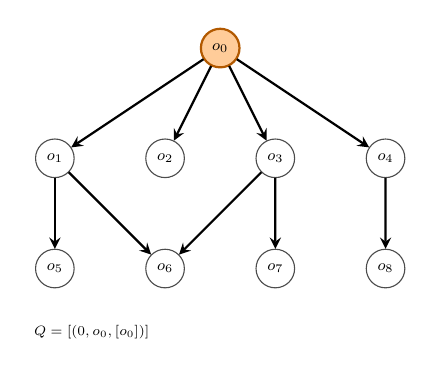
\begin{tikzpicture}[
    scale=0.7, transform shape,
    every node/.style={circle, draw, minimum size=7mm, font=\footnotesize\ttfamily},
    edge/.style={draw, ->, >=stealth, thick},
    current/.style={fill=orange!40, draw=orange!70!black, thick},
    default/.style={fill=white, draw=gray!60!black}
]
% Level 0
\node[current] (o0) at (3,4) {$o_0$};

% Level 1
\node[default] (o1) at (0,2) {$o_1$};
\node[default] (o2) at (2,2) {$o_2$};
\node[default] (o3) at (4,2) {$o_3$};
\node[default] (o4) at (6,2) {$o_4$};

% Level 2
\node[default] (o5) at (0,0) {$o_5$};
\node[default] (o6) at (2,0) {$o_6$};
\node[default] (o7) at (4,0) {$o_7$};
\node[default] (o8) at (6,0) {$o_8$};

% Edges from o0
\draw[edge] (o0) -- (o1);
\draw[edge] (o0) -- (o2);
\draw[edge] (o0) -- (o3);
\draw[edge] (o0) -- (o4);

% Edges from Level 1 to Level 2
\draw[edge] (o1) -- (o5);
\draw[edge] (o1) -- (o6);
\draw[edge] (o3) -- (o6);
\draw[edge] (o3) -- (o7);
\draw[edge] (o4) -- (o8);

% Queue annotation
\node[draw=none, rectangle, anchor=north west, align=left, font=\scriptsize, text=black]
    at (-0.5,-0.8) {$Q = [(0, o_0, [o_0])]$};
\end{tikzpicture}

        \label{fig:bfs_step_a}
    }
    \hfill
    \subfloat[Expand $o_0$ - candidates.]{
        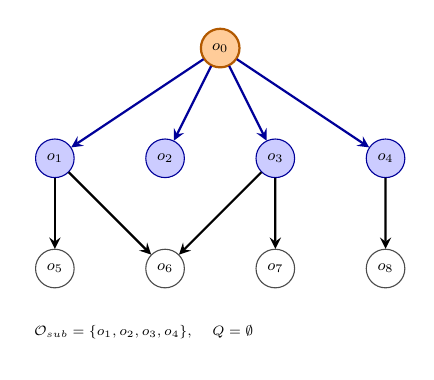
\begin{tikzpicture}[
    scale=0.7, transform shape,
    every node/.style={circle, draw, minimum size=7mm, font=\footnotesize\ttfamily},
    edge/.style={draw, ->, >=stealth, thick},
    candidedge/.style={draw, ->, >=stealth, thick, blue!60!black},
    current/.style={fill=orange!40, draw=orange!70!black, thick},
    candidate/.style={fill=blue!20, draw=blue!60!black},
    default/.style={fill=white, draw=gray!60!black}
]
% Level 0
\node[current] (o0) at (3,4) {$o_0$};

% Level 1 - all candidates (blue)
\node[candidate] (o1) at (0,2) {$o_1$};
\node[candidate] (o2) at (2,2) {$o_2$};
\node[candidate] (o3) at (4,2) {$o_3$};
\node[candidate] (o4) at (6,2) {$o_4$};

% Level 2
\node[default] (o5) at (0,0) {$o_5$};
\node[default] (o6) at (2,0) {$o_6$};
\node[default] (o7) at (4,0) {$o_7$};
\node[default] (o8) at (6,0) {$o_8$};

% Candidate edges from o0 (blue)
\draw[candidedge] (o0) -- (o1);
\draw[candidedge] (o0) -- (o2);
\draw[candidedge] (o0) -- (o3);
\draw[candidedge] (o0) -- (o4);

% Edges from Level 1 to Level 2 (default)
\draw[edge] (o1) -- (o5);
\draw[edge] (o1) -- (o6);
\draw[edge] (o3) -- (o6);
\draw[edge] (o3) -- (o7);
\draw[edge] (o4) -- (o8);

% Annotation
\node[draw=none, rectangle, anchor=north west, align=left, font=\scriptsize, text=black]
    at (-0.5,-0.8) {$\mathcal{O}_{\text{sub}} = \{o_1, o_2, o_3, o_4\}$, \quad $Q = \emptyset$};
\end{tikzpicture}

        \label{fig:bfs_step_b}
    }\\[2mm]
    \subfloat[Expand $o_0$ - selection.]{
        \begin{tikzpicture}[
    scale=0.7, transform shape,
    every node/.style={circle, draw, minimum size=7mm, font=\footnotesize\ttfamily},
    edge/.style={draw, ->, >=stealth, thick},
    selectedge/.style={draw, ->, >=stealth, very thick, green!60!black},
    rejectededge/.style={draw, ->, >=stealth, thick, gray!50,
        decoration={markings, mark=at position 0.5 with {\node[red, font=\scriptsize\bfseries, draw=none, fill=none] {$\times$};}},
        postaction={decorate}},
    processed/.style={fill=green!30, draw=green!60!black, thick},
    queued/.style={fill=green!15, draw=green!60!black, dashed, thick},
    rejected/.style={fill=gray!30, draw=gray!60!black},
    default/.style={fill=white, draw=gray!60!black}
]
% Level 0
\node[processed] (o0) at (3,4) {$o_0$};

% Level 1
\node[queued] (o1) at (0,2) {$o_1$};
\node[rejected] (o2) at (2,2) {$o_2$};
\node[queued] (o3) at (4,2) {$o_3$};
\node[rejected] (o4) at (6,2) {$o_4$};

% Level 2
\node[default] (o5) at (0,0) {$o_5$};
\node[default] (o6) at (2,0) {$o_6$};
\node[default] (o7) at (4,0) {$o_7$};
\node[default] (o8) at (6,0) {$o_8$};

% Selected edges from o0
\draw[selectedge] (o0) -- (o1);
\draw[selectedge] (o0) -- (o3);

% Rejected edges from o0
\draw[rejectededge] (o0) -- (o2);
\draw[rejectededge] (o0) -- (o4);

% Edges from Level 1 to Level 2 (default)
\draw[edge] (o1) -- (o5);
\draw[edge] (o1) -- (o6);
\draw[edge] (o3) -- (o6);
\draw[edge] (o3) -- (o7);
\draw[edge] (o4) -- (o8);

% Annotation
\node[draw=none, rectangle, anchor=north west, align=left, font=\scriptsize, text=black]
    at (-0.5,-0.8) {$\mathcal{D}(\{o_1,o_2,o_3,o_4\}) \to \{o_1,o_3\}$\\$Q = \{(1, o_1, [o_0,o_1]), (1, o_3, [o_0,o_3])\}$};
\end{tikzpicture}

        \label{fig:bfs_step_c}
    }
    \hfill
    \subfloat[Expand $o_1$ - candidates.]{
        \input{graphics/tikz/bfs_step_d.tex}
        \label{fig:bfs_step_d}
    }\\[2mm]
    \subfloat[Expand $o_1$ - selection.]{
        \begin{tikzpicture}[
    scale=0.7, transform shape,
    every node/.style={circle, draw, minimum size=7mm, font=\footnotesize\ttfamily},
    edge/.style={draw, ->, >=stealth, thick},
    selectedge/.style={draw, ->, >=stealth, very thick, green!60!black},
    rejectededge/.style={draw, ->, >=stealth, thick, gray!50,
        decoration={markings, mark=at position 0.5 with {\node[red, font=\scriptsize\bfseries, draw=none, fill=none] {$\times$};}},
        postaction={decorate}},
    processed/.style={fill=green!30, draw=green!60!black, thick},
    queued/.style={fill=green!15, draw=green!60!black, dashed, thick},
    rejected/.style={fill=gray!30, draw=gray!60!black},
    default/.style={fill=white, draw=gray!60!black}
]
% Level 0
\node[processed] (o0) at (3,4) {$o_0$};

% Level 1
\node[processed] (o1) at (0,2) {$o_1$};
\node[rejected] (o2) at (2,2) {$o_2$};
\node[queued] (o3) at (4,2) {$o_3$};
\node[rejected] (o4) at (6,2) {$o_4$};

% Level 2
\node[rejected] (o5) at (0,0) {$o_5$};
\node[queued] (o6) at (2,0) {$o_6$};
\node[default] (o7) at (4,0) {$o_7$};
\node[default] (o8) at (6,0) {$o_8$};

% Selected edges from o0
\draw[selectedge] (o0) -- (o1);
\draw[selectedge] (o0) -- (o3);

% Rejected edges from o0
\draw[rejectededge] (o0) -- (o2);
\draw[rejectededge] (o0) -- (o4);

% Edges from o1
\draw[selectedge] (o1) -- (o6);
\draw[rejectededge] (o1) -- (o5);

% Default edges from o3
\draw[edge] (o3) -- (o6);
\draw[edge] (o3) -- (o7);

% Rejected edge from o4
\draw[rejectededge] (o4) -- (o8);

% Annotation
\node[draw=none, rectangle, anchor=north west, align=left, font=\scriptsize, text=black]
    at (-0.5,-0.8) {$\mathcal{D}(\{o_5,o_6\}) \to \{o_6\}$\\$Q = \{(1, o_3, [o_0,o_3]), (2, o_6, [o_0,o_1,o_6])\}$};
\end{tikzpicture}

        \label{fig:bfs_step_e}
    }
    \hfill
    \subfloat[Expand $o_3$ - candidates.]{
        \input{graphics/tikz/bfs_step_f.tex}
        \label{fig:bfs_step_f}
    }\\[2mm]
    \subfloat[Expand $o_3$ - selection.]{
        \input{graphics/tikz/bfs_step_g.tex}
        \label{fig:bfs_step_g}
    }
    \hfill
    \subfloat[Termination.]{
        \begin{tikzpicture}[
    scale=0.7, transform shape,
    every node/.style={circle, draw, minimum size=7mm, font=\footnotesize\ttfamily},
    edge/.style={draw, ->, >=stealth, thick},
    selectedge/.style={draw, ->, >=stealth, very thick, green!60!black},
    rejectededge/.style={draw, ->, >=stealth, thick, gray!50,
        decoration={markings, mark=at position 0.5 with {\node[red, font=\scriptsize\bfseries, draw=none, fill=none] {$\times$};}},
        postaction={decorate}},
    processed/.style={fill=green!30, draw=green!60!black, thick},
    rejected/.style={fill=gray!30, draw=gray!60!black},
    default/.style={fill=white, draw=gray!60!black}
]
% Level 0
\node[processed] (o0) at (3,4) {$o_0$};

% Level 1
\node[processed] (o1) at (0,2) {$o_1$};
\node[rejected] (o2) at (2,2) {$o_2$};
\node[processed] (o3) at (4,2) {$o_3$};
\node[rejected] (o4) at (6,2) {$o_4$};

% Level 2
\node[rejected] (o5) at (0,0) {$o_5$};
\node[processed] (o6) at (2,0) {$o_6$};
\node[processed] (o7) at (4,0) {$o_7$};
\node[rejected] (o8) at (6,0) {$o_8$};

% Selected path edges
\draw[selectedge] (o0) -- (o1);
\draw[selectedge] (o0) -- (o3);
\draw[selectedge] (o1) -- (o6);
\draw[selectedge] (o3) -- (o6);
\draw[selectedge] (o3) -- (o7);

% Rejected edges
\draw[rejectededge] (o0) -- (o2);
\draw[rejectededge] (o0) -- (o4);
\draw[rejectededge] (o1) -- (o5);
\draw[rejectededge] (o4) -- (o8);

% Annotation
\node[draw=none, rectangle, anchor=north west, align=left, font=\scriptsize, text=black]
    at (-0.5,-0.8) {$Q = \emptyset$, \quad $\mathcal{P} = \{[o_0,o_1,o_6], [o_0,o_3,o_6], [o_0,o_3,o_7]\}$};
\end{tikzpicture}

        \label{fig:bfs_step_h}
    }

    \caption{Breadth-first traversal on an ontology DAG. Node states: \textcolor{orange!70!black}{orange} = expanding, \textcolor{blue!60!black}{blue} = candidate, \textcolor{green!60!black}{green solid} = processed, \textcolor{green!60!black}{green dashed} = queued, \textcolor{gray}{gray} = rejected. Rejected edges are marked with \textcolor{red}{$\times$}.}
    \label{fig:bfs_example}
\end{figure}

Figure~\ref{fig:bfs_example} illustrates the traversal on an ontology rooted at $o_0$ with two subclass layers. Consider annotating a column with header \textit{Fuel Type} from an energy dataset, with sample values such as \texttt{diesel}, \texttt{gasoline}, and \texttt{natural gas}. Let $l_{\max}=2$. The queue evolution is as follows:

\begin{enumerate}
    \item \textbf{Initialization (Fig.~\ref{fig:bfs_step_a}).}
    Initialize $\mathcal{P}\leftarrow\emptyset$ and $Q\leftarrow\emptyset$; enqueue $(0,o_0,[o_0])$.
    Queue state: $Q = [(0, o_0, [o_0])]$.

    \item \textbf{Expanding $o_0$ - candidate phase (Fig.~\ref{fig:bfs_step_b}).}
    Dequeue $(0,o_0,[o_0])$ and retrieve $\mathcal{O}_{\text{sub}}(o_0)=\{o_1,o_2,o_3,o_4\}$.
    These four subclasses (shown in blue) are passed to the decision module $\mathcal{D}$ for evaluation.

    \item \textbf{Expanding $o_0$ - selection result (Fig.~\ref{fig:bfs_step_c}).}
    The decision module returns $\mathcal{O}_{\text{sel}}=\{o_1,o_3\}$, rejecting $o_2$ and $o_4$.
    Enqueue $(1,o_1,[o_0,o_1])$ and $(1,o_3,[o_0,o_3])$.
    Queue state: $Q = [(1, o_1, [o_0,o_1]), (1, o_3, [o_0,o_3])]$.
    Selected nodes are shown with dashed green borders; rejected edges are marked with a red $\times$.

    \item \textbf{Expanding $o_1$ - candidate phase (Fig.~\ref{fig:bfs_step_d}).}
    Dequeue $(1,o_1,[o_0,o_1])$ and retrieve $\mathcal{O}_{\text{sub}}(o_1)=\{o_5,o_6\}$.
    These two subclasses (shown in blue) are passed to $\mathcal{D}$ for evaluation.
    Note that $o_3$ remains in the queue (dashed green), awaiting its turn.

    \item \textbf{Expanding $o_1$ - selection result (Fig.~\ref{fig:bfs_step_e}).}
    The decision module selects $\{o_6\}$ and rejects $o_5$.
    Enqueue $(2,o_6,[o_0,o_1,o_6])$.
    Queue state: $Q = [(1, o_3, [o_0,o_3]), (2, o_6, [o_0,o_1,o_6])]$.

    \item \textbf{Expanding $o_3$ - candidate phase (Fig.~\ref{fig:bfs_step_f}).}
    Dequeue $(1,o_3,[o_0,o_3])$ and retrieve $\mathcal{O}_{\text{sub}}(o_3)=\{o_6,o_7\}$.
    These two subclasses are passed to $\mathcal{D}$ for evaluation.
    Note that $o_6$ is already queued from $o_1$'s path, but is evaluated again under $o_3$'s context.

    \item \textbf{Expanding $o_3$ - selection result (Fig.~\ref{fig:bfs_step_g}).}
    The decision module selects both $\{o_6,o_7\}$.
    Enqueue $(2,o_6,[o_0,o_3,o_6])$ and $(2,o_7,[o_0,o_3,o_7])$.
    Queue state: $Q = [(2, o_6, [o_0,o_1,o_6]), (2, o_6, [o_0,o_3,o_6]), (2, o_7, [o_0,o_3,o_7])]$.

    \item \textbf{Termination (Fig.~\ref{fig:bfs_step_h}).}
    All remaining queue elements have depth $2=l_{\max}$, so the traversal finalizes each path without further expansion.
    The output is $\mathcal{P}=\{[o_0,o_1,o_6],\,[o_0,o_3,o_6],\,[o_0,o_3,o_7]\}$.
\end{enumerate}

The endpoint class $o_6$ appears under two distinct paths, reflecting that multiple higher-level categories can legitimately contextualize the same fine-grained label. The next section introduces ranking and consolidation strategies that control this multiplicity under scalability constraints.

\section{Chain-of-Thought Prompt Engineering}
\label{sec:prompt_engineering}

CTA in this pipeline relies on large language models (LLMs) to evaluate semantic compatibility between column evidence and ontology candidates. However, unconstrained LLM generations can be inconsistent and may produce labels not present in the ontology. The method therefore uses a structured prompting procedure that constrains the output space while eliciting intermediate reasoning steps, commonly known as chain-of-thought (CoT) prompting~\cite{wei2022chain}.

The prompt structure consists of three key components:

\begin{enumerate}
    \item \textbf{Role Definition:} The system message defines the LLM's role as an expert in semantic table annotation, with the goal of selecting the most appropriate ontology class for a given column based on the provided metadata.
    \item \textbf{Contextual Evidence:} To ground the model's decision, the prompt includes serialized table context (table name, column headers, and sample rows) formatted in Markdown. This provides the necessary evidence for disambiguating generic column names (e.g., distinguishing a numerical ``Capacity'' column as either electrical generation capacity or volume).
    \item \textbf{Constrained Candidate Set:} Crucially, the BFS traversal (Section~\ref{sec:bfs}) dynamically supplies a limited set of valid ontology classes ($\mathcal{O}_{\text{sub}}$) available at the current depth. The LLM is restricted to choosing from this set (or one of their ancestors), effectively transforming open-ended generation into a multiple-choice classification task grounded in the ontology.
\end{enumerate}

\paragraph{Implementation}
To improve the robustness of semantic judgments, the prompt separates the output into two logical blocks: a reasoning block and a final-answer block. Concretely, the prompt instructs the model to:
\begin{quote}
    ``First, output your reasoning enclosed in \texttt{<reasoning>...</reasoning>} tags. Then output the final answer enclosed in \texttt{<answer>...</answer>} tags.''
\end{quote}

The separation encourages an explicit justification of the relationship between column values and candidate classes before committing to a label. Within the \texttt{<reasoning>...</reasoning>} block, the model typically analyzes value patterns (e.g., \texttt{Solar} under a \texttt{Fuel} column suggests a renewable energy source) and contrasts candidate definitions. The extracted content of the \texttt{<answer>...</answer>} block is then parsed for the subsequent Ensemble Decision-Making phase.


\section{LLM-based Ensemble Decision-Making}
\label{sec:edm}

The decision module $\mathcal{D}$ in Algorithm~\ref{alg:bfs} determines which candidate classes to retain at each BFS level. Single LLM calls can be inconsistent, can hallucinate ontology-incompatible labels, and can be truncated by context-window limits. The pipeline therefore uses an \emph{Ensemble Decision-Making} (EDM) strategy that aggregates votes from multiple independent LLM agents to improve robustness.

The EDM module is governed by three hyperparameters: $\alpha$ (\emph{agents per class}) specifies how many independent agents evaluate each candidate class; $\beta$ (\emph{classes per agent}) bounds the workload assigned to a single agent; and $\theta \in [0,1]$ (\emph{consensus threshold}) sets the minimum vote ratio required for a class to be selected. The number of agents $n$ is computed dynamically to balance evaluation coverage and computational cost:
\begin{equation}
n = \max\left(\alpha,\, \left\lfloor\frac{|\hat{\mathcal{O}}| \cdot \alpha}{\beta}\right\rfloor + 1\right)
\label{eq:num_agents}
\end{equation}
This formula ensures that (i) at least $\alpha$ agents are available so each class can receive the required number of evaluations, and (ii) no agent is overloaded beyond $\beta$ classes on average.

\begin{algorithm}[htb]
\caption{LLM-based Ensemble Decision-Making}
\label{alg:edm}
\KwIn{
    Table context: name $t_n$, header $t_h$, sample rows $t_d$; \\
    Target column $c$; Candidate classes $\hat{\mathcal{O}}$; \\
    Agents per class $\alpha$; Classes per agent $\beta$; Consensus threshold $\theta$
}
\KwOut{Selected classes $\mathcal{O}_{\text{sel}} \subseteq \hat{\mathcal{O}}$}

\tcp{Step 1: Compute number of agents}
$n \leftarrow \max\bigl(\alpha,\, \lfloor|\hat{\mathcal{O}}| \cdot \alpha / \beta\rfloor + 1\bigr)$\;
Initialize assignment lists: $\text{assigned}[i] \leftarrow \emptyset$ for $i \in \{1, \ldots, n\}$\;
Initialize counters: $\text{votes}[o] \leftarrow 0$, $\text{seen}[o] \leftarrow 0$ for all $o \in \hat{\mathcal{O}}$\;

\BlankLine
\tcp{Step 2: Assign classes to agents}
\For{each class $o \in \hat{\mathcal{O}}$}{
    $\mathcal{I}_o \leftarrow$ randomly select $\min(\alpha, n)$ indices from $\{1, \ldots, n\}$\;
    \For{each $j \in \mathcal{I}_o$}{
        $\text{assigned}[j] \leftarrow \text{assigned}[j] \cup \{o\}$\;
        $\text{seen}[o] \leftarrow \text{seen}[o] + 1$\;
    }
}

\BlankLine
\tcp{Step 3: Query agents in parallel}
\ForPar{$i \leftarrow 1$ \KwTo $n$}{
    \If{$\text{assigned}[i] \neq \emptyset$}{
        $Q_i \leftarrow \textsc{GeneratePrompt}(t_n, t_h, t_d, c, \text{assigned}[i])$\;
        $R_i \leftarrow \textsc{LLMQuery}(Q_i)$\;
        $V_i \leftarrow \textsc{ParseAnswer}(R_i) \cap \text{assigned}[i]$\;
        \For{each $o \in V_i$}{
            $\text{votes}[o] \leftarrow \text{votes}[o] + 1$\;
        }
    }
}

\BlankLine
\tcp{Step 4: Apply consensus threshold}
$\mathcal{O}_{\text{sel}} \leftarrow \emptyset$\;
\For{each class $o \in \hat{\mathcal{O}}$}{
    \If{$\text{votes}[o] > 0$ \textbf{and} $\text{votes}[o] / \text{seen}[o] \geq \theta$}{
        $\mathcal{O}_{\text{sel}} \leftarrow \mathcal{O}_{\text{sel}} \cup \{o\}$\;
    }
}
\Return $\mathcal{O}_{\text{sel}}$\;
\end{algorithm}

Algorithm~\ref{alg:edm} proceeds in four phases. First, the number of agents $n$ is determined according to Equation~\ref{eq:num_agents}. Second, each candidate class $o \in \hat{\mathcal{O}}$ is randomly assigned to $\min(\alpha, n)$ agents; the counter $\text{seen}[o]$ records how many agents will evaluate class $o$. Third, all agents query the LLM in parallel with their assigned subsets of classes. Each agent constructs a prompt containing the table context (name, headers, sample rows), the target column, and its assigned candidates. The LLM response is parsed to extract the classes the agent deems relevant, and only classes within the agent's assignment are counted as votes. Finally, a class is selected if and only if it receives at least one positive vote and the ratio of votes to evaluating agents meets or exceeds the consensus threshold~$\theta$.

Agent queries are independent and therefore parallelizable: each agent issues an LLM request for its assigned subset of classes. With sufficient API concurrency, parallel execution reduces wall-clock latency from $O(n)$ sequential calls to $O(1)$ parallel calls. The additional constraint $\text{votes}[o] > 0$ in line~24 prevents vacuous acceptance when all evaluating agents abstain from voting for a particular class. Together, ontology-driven traversal, constrained prompting, and EDM yield a scalable CTA pipeline for heterogeneous energy tables.
